\documentclass[
 reprint,
 amsmath,amssymb,
 aps,
]{revtex4-1}

\usepackage{graphicx}  
\usepackage{epstopdf}
\usepackage{dcolumn}
\usepackage{bm}	
\usepackage{amsmath}			
\usepackage{amsfonts}			
\usepackage{amssymb}			
\usepackage{latexsym}		
\usepackage{color}
\usepackage{ stmaryrd }
\begin{document}

\title{Kinetic plasma response to the forward stimulated Brillouin scattering and impact on  the propagation of  energetic laser pulses}
\author{C. Ruyer}\email{charles.ruyer@cea.fr}
\author{A. Debayle}
\author{P. Loiseau}
\author{M. Casanova}
\author{P. E. Masson-Laborde}
\affiliation{CEA, DAM, DIF, F-91297 Arpajon, France}

\begin{abstract}
We address the scattering of a high energy laser pulse on a   large wavelength acoustic turbulence of relevance for LMJ or NIF-class  experiments. A kinetic description, accounting correctly for the plasma acoustic  response to driven perturbation, is adopted and combined with a linearized and paraxial  description of the laser propagation including diffraction. We could evidence that a rear-focus and  a far prior-focus region   can be unstable to the growth of an electromagnetic wave of wavevector close to the pump's, possibly leading to the strong deformation of the intensity pattern and resulting energy deposition. 
\end{abstract}

\maketitle

\section{Introduction}
\begin{itemize}
    \item high energy density physics is very cool very  fun and very interesting.
    \item It requires the precise predictions of the  laser propagation  along with parametric instabilities and their coupling with the smoothing technics, routinely used in high energy class facilities.  
    \item Forward instabilities such as filamentation, forward Brillouin  or plasma smoothing effects \cite[]{ POP_Grech_2006,PRL_Grech_2009} are vastly unexplored, and let's be honest, far more complicated than playing ping pong with positrons.
\end{itemize}

High energy class laser facilities such as LMJ or  NIF \cite[]{}  routinely bring matter under extreme conditions, not only of interest for inertial confinement fusion \cite{Lindl_2004,He_2007,Cavailler_2005}, but also for high energy astrophysics \cite{Drake_2012} and high energy density physics   \cite{Drake2006}. 
Whether  the laser   serves as heat source or as a diagnostics, the accurate prediction of its propagation remain crucial for understanding  the experiment outputs. 



We address in this publication the theoretical description of  the growth of an electromagnetic wave of wavevector and frequency close to the pump wave's and in a driven acoustic turbulence described in a kinetic framework. 
Our stimulated forward Brillouin scattering (FSBS) model    evidences the crucial kinetic response of the plasma to the acoustic waves driven by the beating between the non-monochromatic pump and scattered beam. 
Combining a linearize paraxial description of light, an asymptotic (in time) plasma  response and a simple model of Random Phase Plate (RPP) smoothed laser beam, we derived, after a bloody year of brain teasing torture, a predictive perturbative model that could pinpoint the significant growth and intensity pattern modification relevant for NIF or LMJ-class experiments. 
Due to a fanatic stubbornness crowned by a confinement cutting off any super-computer entertainment, we could extract an effective spatial growth rate with its dependence on the scattering directions and position relative to the focal plane. 
The last section gather our perspective and concluding remarks. 

\section{Paraxial propagation of an RPP beam in a driven acoustic turbulence}
\subsection{Pump wave and diffusion of  laser fields}
Following the developments of Refs. \cite[]{phd-Grech}, we start by an electric field with a main propagation direction lying on the $x$-axis and a broad transverse spatial spectrum with two frequencies, $\omega_p$ and $\omega_d$ for the pump and diffused wave  respectively.  Note that the vectors are noted in bold symbols throughout this study. Introducing, $D=1$ or $2$, the number of transverse directions, we assume that the electric field in real space that depends on space and time, $\mathbf{r}$  and $t$ respectively, reads
\begin{align}
E(\mathbf{r},t)= \Re \Big[ \int \frac{d^Dk_p}{(2\pi)^D} E_p (\mathbf{k}_p,t) e^{i \mathbf{k}_p \cdot \mathbf{r}_\perp} \nonumber \\
+\int \frac{d^Dk_d}{(2\pi)^D} E_d (\mathbf{k}_d,t) e^{i \mathbf{k}_d \cdot \mathbf{r}_\perp -i (\omega_d - \omega_p)t}   \Big] \, ,
\end{align}
where the subscript $\perp$ designate the transverse direction [$(y,z)$ and $y$ in three and two dimension respectively]  components and $\Re$  ($\Im$) the real (imaginary) part of a complex. Note that the electric field, as written above,  has already been enveloped in time and space around $\omega_p$ and $k_0$ so that the physical one should be multiplied  by $\exp(ik_0 x-i\omega_p t)$ (with $i^2=-1$).

In the transverse Fourier space, dropping the dependence in time and $x$ for simplicity and with $\omega_s=\omega_d - \omega_p$,
\begin{align}
E(\mathbf{k}) =     E_p(\mathbf{k})
+  E_d(\mathbf{k}) e^{ -i \omega_s t}   \, .
\end{align} 
Using $I(k)=c\epsilon_0 \int E(k_p) E(k-k_p) dk_p$, we may split the total intensity in a pump intensity $I_p$ and diffused one $I_d$ verifying to leading order in $E_d$, \emph{i.e.} for $\vert E_d\vert \ll \vert E_p \vert$, 
\begin{align}
I(\mathbf{k}) &=I_p(\mathbf{k})+I_d(\mathbf{k})\, , \label{eq:itot}\\
I_p(\mathbf{k}_p) &=   \frac{c\epsilon_0}{2} \int E_p(\mathbf{k}) E_p^\star(\mathbf{k}_p-\mathbf{k}) d^Dk \, , \label{eq:ip} \\
I_d(\mathbf{k}_d) &\simeq   c\epsilon_0  \Re \int E_p(\mathbf{k}) E_d^\star(\mathbf{k}_d-\mathbf{k})e^{i\omega_s t } d^Dk \, , \label{eq:id}
\end{align}
with $\epsilon_0$ and  $c$, the electric permittivity and speed of light in vacuum.
In this study we will only consider wavevectors cloth to the initial
propagation direction ($x$) and note $\mathbf{k}_{p/d}=k_0\hat{\mathbf{x}} +k_{p/d,\perp}\hat{\mathbf{r}_\perp}  $ where $\hat{\mathbf{x}}$ and $\hat{\mathbf{r}_\perp}$ are unity vectors in the $x$ and transverse directions respectively. Hence, $\omega_p^2 = \omega_{pe}^2+ \mathbf{k}_p^2c^2$ and $\omega_d^2 = \omega_{pe}^2+\mathbf{k}_d^2c^2$ where $\omega_{ps}$ is the $s$-species plasma frequency and the susbscripts $e,i$ corresponds the the electrons and ions respectively.

Hence, for a pump  diffusion that occurs close to the $x$-axis,  \emph{i.e.}  $\vert \mathbf{k}_p -\mathbf{k}_d\vert \ll k_0$ and we may write to leading order the plasma wave frequency and wavevector,
\begin{align}
\omega_s=\omega_p-\omega_d&= -(\mathbf{k}_s^2 c^2-2\mathbf{k}_p\cdot\mathbf{k}_s c^2)/2\omega_0
\, , \nonumber\\
\mathbf{k}_s& = \mathbf{k}_p-\mathbf{k}_d\, ,
\end{align}
where $\omega_0^2= \omega_{pe}^2+ k_0^2c^2$.
Hereafter, we will assume that the plasma wave remains mainly transverse to the pump so that $\mathbf{k}_s=k_s \hat{\mathbf{r}_\perp}$ and $ \vert \mathbf{k}_p\cdot\mathbf{k}_s\vert \ll k_s^2$. 
Hence, use will be made of 
\begin{align}
\omega_s  &= -\frac{k_s^2 c^2 }{2\omega_0} \, ,\label{eq:ws}\\
\frac{\omega_s}{k_s}& = -\frac{k_s c^2 }{2\omega_0} \label{eq:vphis} \, .
\end{align}
Noticing $k_s/k_0\equiv \sin(\theta) $, one recovers the vastly used  relation giving, as a function of the incident angle of two plane waves, the phase speed of the  diffraction pattern of interest in the case of cross-beam energy transfer (CBET) \cite[]{POP_Debayle_2018}.

Introducing the laser critical density, $n_c = m_e \epsilon_0c^2 k_0^2/q_e^2 $ (where  $m_e$ and  $q_e$ are the  electron mass and charge respectively), the  paraxial propagation equation of the electric field verifies \cite[]{POP_Grech_2006}
\begin{equation}
    \partial_x E(t) +\frac{i\mathbf{k}^2}{2k_0}E=\frac{-ik_0n_0}{2n_c} \int \frac{d^Dk_s}{(2\pi)^D} \frac{\delta n(t,\mathbf{k}_s)}{n} E^\star(t,\mathbf{k}-\mathbf{k}_s) \, ,\label{eq:parax}
\end{equation}
which includes diffraction through the second term of the left-hand side.  
The right-hand side models the  diffusion  of the pump wave  on the broad spectrum density fluctuations ($\delta n/n$).

At this stage it is crucial to  account correctly for the plasma response to the beating between  the pump and the diffused electromagnetic wave. 

\subsection{Plasma response to a driven wave}
\label{sec:drake}
As will be shown subsequently, no monochromatic approximation can be made regarding $E_d(k_d)$ or $\delta n(k_s)/n$, like for the cases of backward Brillouin scattering. Instead, the density fluctuations are the  result of the superposition of many diffraction patterns characterized by there wavevector $k_s$ and with different  phase speeds [see Eq. \eqref{eq:vphis}].

For a given set of $k_p$, $k_s$, $\omega_p$ and $\omega_s$, Eq. (12) of  Ref. \cite[]{POF_Drake_1973} shows that  for  a Maxwellian plasma, the plasma response to a drive  takes on 
\begin{align}
 \frac{ \delta n (\omega_s, k_p,k_s) }{n}  &=   \frac{ -\epsilon_0 E_p(k_p) E_d^\star(k_p-k_s) }{ 4 n_c T_e } \nonumber \\  &\times \alpha_\mathrm{kin}\left(\frac{\omega_s- \mathbf{k}_s\cdot \mathbf{v}_d}{\vert \mathbf{k}_s \vert }\right)   \, ,\label{eq:drake}
 \end{align}
 where, for an ion Debye length $\lambda_{Di}$ that verifies $\vert k_s \lambda_{Di} \vert \ll 1$, %in the case of only one transverse direction ($D=1$), 
 \begin{align}
\alpha_\mathrm{kin} &=  \frac{-1}{2}\frac{ \mathcal{Z}'( \xi_e)\mathcal{Z}'( \xi_i)    }{   \mathcal{Z}'( \xi_i) + \mathcal{Z}'( \xi_e)\frac{  T_i }{ ZT_e } }    \, , \label{eq:drakea}\\
\xi_{e/i } &=  \sqrt{ \frac{ m_{e/i } }{ 2T_{e/i }}  } \left( \frac{ -\vert \mathbf{k}_s\vert c^2  }{  2\omega_0 }  - \frac{    \mathbf{k}_s \cdot \mathbf{v}_d }{  \vert \mathbf{k}_s\vert }\right)  \label{eq:xiie}   \,  .
%\xi_{e/i } &=  \sqrt{ \frac{ m_{e/i } }{ 2T_{e/i }}  } \left( \frac{ -\vert \mathbf{k}_s\vert c^2  }{  2\omega_0 }+\frac{  2\mathbf{k}_{p,\perp}\cdot \mathbf{k}_sc^2 }{  2\vert k_s \vert \omega_0 }  - \frac{    \mathbf{k}_s \cdot \mathbf{v}_d }{  \vert \mathbf{k}_s\vert }\right)  \label{eq:xiie}   \,  .
\end{align}
We introduced $Z$, the ion charge number and  $ \mathcal{Z}$, the plasma dispersion function \cite{Fried_Gell-Mann_1960} and its arguments $\xi_{e } $ and $\xi_{i }$, which in turns depend on $T_{e,i}$ and $v_d$, the electron/ion temperature and  drift velocity.

In order to be combined with the paraxial description of light propagation of Eq. \eqref{eq:parax}, one needs to apply in temporal inverse Fourier transform of Eq. \eqref{eq:drake}. We will account for both stokes $\omega=\omega_s$ and anti-stokes modes $\omega=-\omega_s$ giving 
\begin{equation}\label{eq:sa}
     \frac{ \delta n (t) }{n}= \frac{ \delta n (\omega_s) }{n}e^{-i\omega_st} + \frac{ \delta n (-\omega_s) }{n}e^{i\omega_st}\, .
\end{equation}

We may now use $\alpha_\mathrm{kin}(-u) = \alpha^\star_\mathrm{kin}(u) $ if $u$ is real to recast the above formula as 
\begin{align}
\frac{ \delta n (t,\mathbf{k}_p,\mathbf{k}_s ) }{n}  &=   \frac{ -\epsilon_0 E_p(\mathbf{k}_p) E_d^\star(\mathbf{k}_p-\mathbf{k}_s)  }{ 2 v_g n_c T_e } 
 \Re \left[ \alpha_\mathrm{kin}  e^{ i\omega_s(\mathbf{k}_s) t} \right]  \, .\label{eq:drakef}
\end{align}

Note that the term inside the real part only depends on $k_s$:   a summation of the above relation over $k_p$ results, using Eq. \eqref{eq:id}, in  
\begin{align}
\frac{ \delta n (t,\mathbf{k}_s ) }{n}  &=   \frac{ -I_d(\mathbf{k}_s) }{ 2 v_g n_c T_e } 
 \Re \left( \alpha_\mathrm{kin}   \right)  
 %+ \mathcal{N}(t,\mathbf{k}_s)
 \, .\label{eq:drakef}
\end{align}
%We added to the above equation a seed term, $\mathcal{N}$, that could either come from thermal fluctuations or from an not fully controlled plasma initial condition.  
\begin{figure*}
\begin{tabular}{cc}
(a) $D=1$&
(b) $D=2$, $T_e=1$ keV, $ZT_e/T_i=3$\\
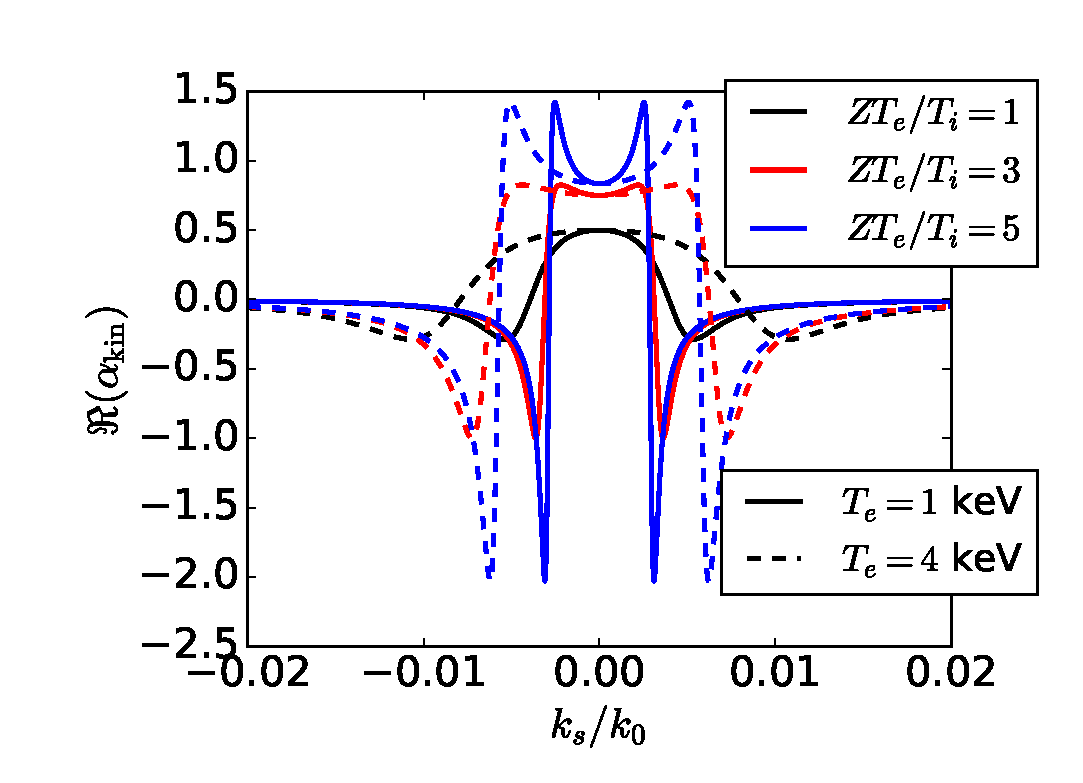
\includegraphics[width=0.49\textwidth]{akin.eps}&
\includegraphics[width=0.49\textwidth]{akinD2.png}
\end{tabular}
\caption{ \label{fig:akin}  
 $\Re \left( \alpha_\mathrm{kin}   \right)$ for $D=1$ (a) and $D=2$ (b) as function of $k_s/k_0$ for a H$^{+}$ plasma with $n_0=0.1n_c$, $T_e =1$ keV for various $ZT_e/T_i$. 
 }
\end{figure*}
In a 2D system ($D=1$), Fig. \ref{fig:akin} illustrates, for $D=1$ and for  a H$^{+}$ plasma with $n_0=0.1n_c$ and  $T_e =1$ keV, that $\Re \left( \alpha_\mathrm{kin}   \right)$ is an even function  of $k_s/k_0$ of width that enlarges as  $T_e$ increases. Moreover, its value vanishes for $\vert k_s/k_0 \vert  \gtrsim 2 \cdot 10^{-2}$, showing that the plasma is sensitive  to the very large wavelength perturbations ($\lambda_s/\lambda_0=k_0/k_s\gtrsim 314 $ or $k_s/k_0\lesssim 0.02$).
%\textcolor{red}{Asymmetry 2D 3D.}
As there is, in  the system of interest here no privileged scattering direction, both stokes and antistokes plasma response modes have to be taken into account [see Eq. \eqref{eq:sa}]. Hence,  the resulting diffraction pattern  in the case of FSBS is  a stationary  wave, unlike CBET where it is fully propagating.

\subsection{Derivation of an effective growth rate relevant for an  RPP beam}
 \begin{widetext}
We may now combine the kinetic plasma response  with the paraxial model of  the laser propagation. 
However, it  is easier at this stage to introduce $\Bar{E}$ with  $E=\Bar{E}\exp(-i \mathbf{k}^2x /2k_0)$ so that Eq. \eqref{eq:parax} becomes
\begin{equation}
    \partial_x \Bar{E}  =\frac{-ik_0n_0}{2n_c} e^{\frac{i\mathbf{k}^2x }{2k_0}}\int \frac{d^Dk_s}{(2\pi)^D} \frac{\delta n(\mathbf{k}_s)}{n} \Bar{E}^\star(\mathbf{k}-\mathbf{k}_s) e^{ \frac{i(\mathbf{k}-\mathbf{k}_s)^2x}{2k_0}}\, ,  \label{eq:paraxbar}
\end{equation}
 plugged in Eq. \eqref{eq:drakef}, we obtain
\begin{align}
    \partial_x \Bar{E}  =\frac{ik_0n_0}{4n_c} \frac{e^{\frac{i\mathbf{k}^2 x}{2k_0}}}{  v_g n_c T_e}
    %\times \nonumber \\
    \int \frac{d^Dk_s}{(2\pi)^D}  e^{ \frac{i(\mathbf{k}-\mathbf{k}_s)^2x}{2k_0}} \Bar{E}^\star(\mathbf{k}-\mathbf{k}_s) 
   I_d(\mathbf{k}_s) \alpha_\mathrm{r}   (\mathbf{k}_s) 
   %-\frac{ik_0n_0}{2n_c} e^{\frac{i\mathbf{k}^2x }{2k_0}}\int \frac{d^Dk_s}{(2\pi)^D} \mathcal{N}(\mathbf{k}_s) \Bar{E}^\star(\mathbf{k}-\mathbf{k}_s) e^{ \frac{i(\mathbf{k}-\mathbf{k}_s)^2x}{2k_0}}
   \, ,  \label{eq:paraxbar}
\end{align}
where we introduced $\alpha_\mathrm{r}=\Re(\alpha_\mathrm{kin} )$. 

%\onecolumngrid
 When retaining only the first order terms (as $E_d$, $I_d$; $I_p$ and $E_p$ are considered of order zero), we obtain 
 \begin{align}
   e^{-i\omega_s t}\partial_x \Bar{E}_d  =&\frac{ik_0n_0}{4n_c} \frac{e^{\frac{i\mathbf{k}^2 x}{2k_0}}}{  v_g n_c T_e} \times 
   \int \frac{d^Dk_s}{(2\pi)^D} 
   e^{ \frac{i(\mathbf{k}-\mathbf{k}_s)^2x}{2k_0}}
   I_d(\mathbf{k}_s) \alpha_\mathrm{r}   (\mathbf{k}_s) \Bar{E}_p^\star(\mathbf{k}-\mathbf{k}_s) %\nonumber\\
    %&-\frac{ik_0n_0}{2n_c} e^{\frac{i\mathbf{k}^2x }{2k_0}}\int \frac{d^Dk_s}{(2\pi)^D} \mathcal{N}(\mathbf{k}_s) \Bar{E}_p^\star(\mathbf{k}-\mathbf{k}_s) e^{ \frac{i(\mathbf{k}-\mathbf{k}_s)^2x}{2k_0}}
   \, .  \label{eq:paraxbar}
\end{align}

In order to shade light on the dependence of the diffusion growth on the laser energy scattering direction, one needs to combine the above relation with the definition of $I_d(\mathbf{k})$ of  Eq. \eqref{eq:id}, which can be recast as,
\begin{align}
%I_p(\mathbf{k}_d) &\simeq  \frac{c\epsilon_0}{2}  \int d^Dk \Bar{E}_p(\mathbf{k})e^{\frac{ -i\mathbf{k}^2x}{2k_0}-i\omega_s t}\Bar{E}_p^\star(\mathbf{k}_d-\mathbf{k})e^{\frac{ i(\mathbf{k}_d-\mathbf{k})^2x}{2k_0}}   \, , \label{eq:ipb} \\
I_d(\mathbf{k}_d) &\simeq  \Re\left[  c\epsilon_0  \int d^Dk \Bar{E}_d(\mathbf{k})
e^{\frac{ -i\mathbf{k}^2x}{2k_0}-i\omega_s t}
\Bar{E}_p^\star(\mathbf{k}_d-\mathbf{k})
e^{\frac{ i(\mathbf{k}_d-\mathbf{k})^2x}{2k_0}} 
\right]  \, . \label{eq:idb} 
\end{align}
Hence
\begin{align}
\partial_xI_d(\mathbf{k}_d)=  &  c\epsilon_0  \Re\left( \int d^Dk e^{-i\omega_st+ \frac{i( \mathbf{k}_d^2-2\mathbf{k}_d\cdot \mathbf{k} )x}{2k_0}} \Bar{E}_p^\star(\mathbf{k}_d-\mathbf{k} )
\left[\partial_x \Bar{E}_d (\mathbf{k}  ) 
+i\frac{  \mathbf{k}_d^2-2\mathbf{k}_d\cdot \mathbf{k}}{2k_0} \Bar{E}_d(\mathbf{k})
\right]  \right)\, , \label{eq:idbdz}
\end{align}
where the variations along $x$ of $\Bar{E}_p$ were neglected. 
The  use of Eq. \eqref{eq:paraxbar} yields, 
\begin{align}
\partial_xI_d(\mathbf{k}_d)\simeq &\Re\Big( \frac{ik_0n_0}{4n_c} \frac{c\epsilon_0 }{  v_g n_c T_e}   \int d^Dk \int \frac{d^Dk_s}{(2\pi)^D} \Bar{E}_p^\star(\mathbf{k}_d-\mathbf{k})
e^{\frac{i(\mathbf{k}-\mathbf{k}_s)^2x}{2k_0} }
e^{\frac{i(\mathbf{k}_d-\mathbf{k})^2x}{2k_0} }
I_d(\mathbf{k}_s) \alpha_\mathrm{r}(\mathbf{k}_s) 
\Bar{E}_p^\star(\mathbf{k}-\mathbf{k}_s) 
 \Big) \nonumber\\
%+& c\epsilon_0  \Re\left(-\frac{ik_0n_0}{2n_c}  \int d^Dk\int \frac{d^Dk_s}{(2\pi)^D} e^{\frac{i( \mathbf{k}_d-\mathbf{k} )^2x}{2k_0}} \Bar{E}_p^\star(\mathbf{k}_d-\mathbf{k} )\mathcal{N}(\mathbf{k}_s) \Bar{E}_p^\star(\mathbf{k}-\mathbf{k}_s) e^{ \frac{i(\mathbf{k}-\mathbf{k}_s)^2x}{2k_0}}  \right) \nonumber\\
& +c\epsilon_0  \Re\left( \int d^Dk e^{-i\omega_s t+\frac{ i( \mathbf{k}_d^2-2\mathbf{k}_d\cdot \mathbf{k} )x}{2k_0}} 
i\frac{  \mathbf{k}_d^2-2\mathbf{k}_d\cdot \mathbf{k}}{2k_0} \Bar{E}_d(\mathbf{k})\Bar{E}_p^\star(\mathbf{k}_d-\mathbf{k} )
  \right)
\, . \label{eq:g1}
\end{align}
Plugging Eq. \eqref{eq:idb} and retaining only the symmetric terms in the quadratures, 
\begin{align}
\partial_xI_d(\mathbf{k}_d)\simeq \Re\Big( \frac{ik_0n_0}{4n_c} \frac{1 }{  v_g n_c T_e}    \int \frac{d^Dk_s}{(2\pi)^D} I_d(\mathbf{k}_s) \alpha_\mathrm{r}(\mathbf{k}_s)
\Tilde{I}_p(\mathbf{k}_d-\mathbf{k}_s)
+\frac{i\mathbf{k}_d^2}{2k_0} I_d 
%- S(\mathbf{k}_d)
\Big)\, , \label{eq:g2}
\end{align}
where we defined 
\begin{align}
\Tilde{I}_p(\mathbf{k}_d-\mathbf{k}_s)  &=  c\epsilon_0  \int d^Dk \Bar{E}_p^\star (\mathbf{k}_d-\mathbf{k})
e^{\frac{ i (\mathbf{k}_d-\mathbf{k})^2x}{2k_0}-i\omega_s t}
\Bar{E}_p^\star(\mathbf{k}-\mathbf{k}_s)
e^{\frac{ i(\mathbf{k}-\mathbf{k}_s)^2x}{2k_0}}   \, . \label{eq:ipt} 
\end{align}
% and 
% \begin{align}
%S(\mathbf{k}_d) =   \frac{ik_0n_0}{n_c} \int \frac{d^Dk_s}{(2\pi)^D}  
%\mathcal{N}(\mathbf{k}_s)\Tilde{I}_p(\mathbf{k}_d-\mathbf{k}_s)
%\, . \label{eq:s} 
%\end{align}
It is important to note that $\Tilde{I}_p$ differs from $I_p$, and, in order to progress, an assumption on the nature of the pump wave has to be made. 

 \subsection{Energy growth of the Forward Brillouin scattering for an RPP beam }
%For symmetric scattering, the last term  of the above equation may be neglected and, defining $\Bar{I}_d$ through $I_d = \Re[\Bar{I}_d\exp(i\mathbf{k}_d^2x/2k_0)]$, one obtains
% \begin{align}
%\partial_x\Bar{I}_d(\mathbf{k}_d)\simeq  \frac{ik_0n_0}{2n_c} \frac{e^{\frac{-i\mathbf{k}_d^2x}{2k_0}} }{  v_g n_c T_e}   
%  \int \frac{d^Dk_s}{(2\pi)^D} \Bar{I}_d(\mathbf{k}_s) \alpha_\mathrm{r}(\mathbf{k}_s) 
%I_p(\mathbf{k}_d-\mathbf{k}_s)
%e^{\frac{i\mathbf{k}_s^2x}{2k_0}} 
%\, . \label{eq:g3}
%\end{align}
%It is essential to notice that, if diffraction had been neglected, thus removing the exponential terms of the above equations, the real part of $\partial_x \Bar{I}_d$ would be vanishing, implying no growth of the scattered wave. Hence, accounting for diffraction, \emph{i.e.} the curvature of the off focus wave front,  is crucial for modeling the Forward stimulated Brillouin scattering.
 Using the  RPP  beam model of Refs. \cite[]{POF_Schmitt_88,POF_Rose_93} in the transverse Fourier space,
 \begin{align}
 \Bar{E}_p(\mathbf{k}) = \frac{E_0}{N} \sum_{n,\vert k_{\perp,y/z}(n)\vert<k_m } e^{i\Phi_{\mathbf{k}_\perp}}\delta(\mathbf{k}  - \mathbf{k}_\perp(n))\, , \label{eq:erpp}
 \end{align}
 where  $N$ is the number of diffracting elements, 
 $\delta(x)$ the Dirac function and the phases $\Phi_{k_y}$,  independent random variables taking the values $0$ or $\pi$ with equal probability.
 For simplicity, we will assume a square phase plate that verifies $k_{\perp,y/z}(n) = n2k_m/N$ with $n$ an integer that verifies $n\in \llbracket - N/2 ,N/2 \rrbracket$. 
 Under these conditions, and for $\langle u\rangle$ representing the statistical average of $u$,  we note   that $\langle\exp(i\Phi_{k_1}+i\Phi_{k_1})\rangle=\delta(k_1-k_2) $ so that  the statistical average  of Eq. \eqref{eq:ip} verifies
   \begin{align}
   \langle I_p(\mathbf{k})\rangle &= I_0 \sigma ^D \mathcal{H}^{(D)}(\mathbf{k})  &\,  \mathrm{with} \, ,\\ 
   \mathcal{H}^{(1)}(\mathbf{k}) &= H(2k_m - \vert k_y \vert ) &\,  \mathrm{in}\, \mathrm{2D} \, ,\\ 
    \mathcal{H}^{(2)}(\mathbf{k}) &=   H(2k_m - \vert k_y \vert ) H(2k_m - \vert k_z \vert ) &\,  \mathrm{in}\, \mathrm{3D} \, .
   \end{align}
We introduced,  $H$ the step function, $k_m=k_0/2f$ with $f$ the effective speckle focal number,  and $\sigma$ the transverse size of the pump wave, \emph{i.e.}, $I_0\sigma^D$ is its initial power.
As, for $\Tilde{I}_p$, its statistical average for an RPP beam reads, 
\begin{align}
\langle \Tilde{I}_p(\mathbf{k}_d-\mathbf{k}_s)\rangle   &=  c\epsilon_0\frac{E_0^2}{N^2}  \int d^Dk 
e^{\frac{ i (\mathbf{k}_d-\mathbf{k})^2x}{2k_0}-i\omega_s t}
e^{\frac{ i(\mathbf{k}-\mathbf{k}_s)^2x}{2k_0}}  
\sum_{\vert k_{1,y/z}\vert,\vert k_{2,y/z}\vert  <k_m}
\langle e^{i\Phi_{\mathbf{k}_1}+i\Phi_{\mathbf{k}_2}}\rangle
\delta(\mathbf{k}_d-\mathbf{k} -\mathbf{k}_2 ) 
\delta(\mathbf{k}-\mathbf{k}_s -\mathbf{k}_1) 
\, . \label{eq:ipt2} 
\end{align}
When  $\mathbf{k}_1=\mathbf{k}_2$, the Dirac functions in right hand side can be recast into 
\begin{align}
\langle e^{i\Phi_{\mathbf{k}_1}+i\Phi_{\mathbf{k}_2}}\rangle\delta(\mathbf{k}_d-\mathbf{k} -\mathbf{k}_2 ) 
\delta(\mathbf{k}-\mathbf{k}_s -\mathbf{k}_1)=
\delta(\mathbf{k}_2 -\mathbf{k}_1)
\mathcal{H}^{(D)}(2\mathbf{k}-2\mathbf{k}_s  )  \delta (\mathbf{k}_d+\mathbf{k}_s -2\mathbf{k} ) \, ,
\end{align}
and thus yields
\begin{align}
\langle \Tilde{I}_p(\mathbf{k}_d-\mathbf{k}_s)\rangle   &=  I_0\sigma^D
e^{\frac{ i(\mathbf{k}_d-\mathbf{k}_s)^2x}{4k_0}}  
\mathcal{H}^{(D)}\left( \mathbf{k}_d-\mathbf{k}_s  \right)
\, . \label{eq:iptf} 
\end{align}
Hereafter, the $\langle  \cdot \rangle$-notation will  me removed for sake of simplicity. 
Equations \eqref{eq:g2} and \eqref{eq:iptf} may now be combined,  
  \begin{align}
\partial_xI_d(\mathbf{k}_d)&\simeq  \Re\left( \frac{ik_0n_0}{2n_c} \frac{ I_0\sigma^D }{  v_g n_c T_e}   
 \int \frac{d^Dk_s}{(2\pi)^D}   \mathcal{H}^{(D)}(\mathbf{k}_d-\mathbf{k}_s) I_d(\mathbf{k}_s) \alpha_\mathrm{r}(\mathbf{k}_s) e^{\frac{ i(\mathbf{k}_d-\mathbf{k}_s)^2x}{4k_0}}  
 %-S(\mathbf{k}_d) 
 \right)
\, . \label{eq:g4}
%\\S(\mathbf{k}_d) &=   \frac{ik_0n_0}{n_c} I_0\sigma^D\int \frac{d^Dk_s}{(2\pi)^D}  \mathcal{H}^{(D)}\left( \mathbf{k}_d-\mathbf{k}_s  \right)\mathcal{N}(\mathbf{k}_s) e^{\frac{ i(\mathbf{k}_d-\mathbf{k}_s)^2x}{4k_0}}  
\end{align}

Since $2k_m$ is much larger than the width of $\alpha_r(k_s)$ ($\Delta k\ll 2k_m$), we may use $\int_{k_d-2k_m}^{k_d+2k_m} X \simeq \mathcal{H}^{(1)}(k_d) \int_{-\infty}^{+\infty}X$. Introducing $\delta n/n_c=n_0I_0/{n_c^2 T_ev_g}$ we obtain, 
 \begin{align}
\partial_xI_d(\mathbf{k}_d)&\simeq  \frac{-k_0}{2} \frac{ \delta n}{n_c}   \sigma^D
 \mathcal{H}^{(D)}(\mathbf{k}_d)
 \int \frac{d^Dk_s}{(2\pi)^D}    I_d(\mathbf{k}_s) \alpha_\mathrm{r}(\mathbf{k}_s)  \sin\left[{\frac{ (\mathbf{k}_d-\mathbf{k}_s)^2x}{4k_0}}  \right]
 %-S(\mathbf{k}_d)
\, ,  \label{eq:g5}
\end{align}
%In order to reach analytical progress, we will assume that $I_d$ is  smoother and larger  than $\alpha_\mathrm{r}(\mathbf{k}_s) 
%\sin[(\mathbf{k}_d^2-\mathbf{k}_s^2)x / 2k_0]$, hence
%\begin{align}\partial_xI_d(\mathbf{k}_d)\simeq  \frac{-k_0}{2} \frac{ \delta n}{n_c}   \sigma^D\mathcal{H}^{(D)}(\mathbf{k}_d) I_d(0) \int \frac{d^Dk_s}{(2\pi)^D}    \alpha_\mathrm{r}(\mathbf{k}_s) \sin\left[{\frac{ (\mathbf{k}_d-\mathbf{k}_s)^2x}{4k_0}}  \right]\, . %\label{eq:dxidkd}
%\end{align}
 
 \begin{figure*}[!]
\begin{tabular}{cc}
(a) $D=1$ &(b) $D=2$ \\
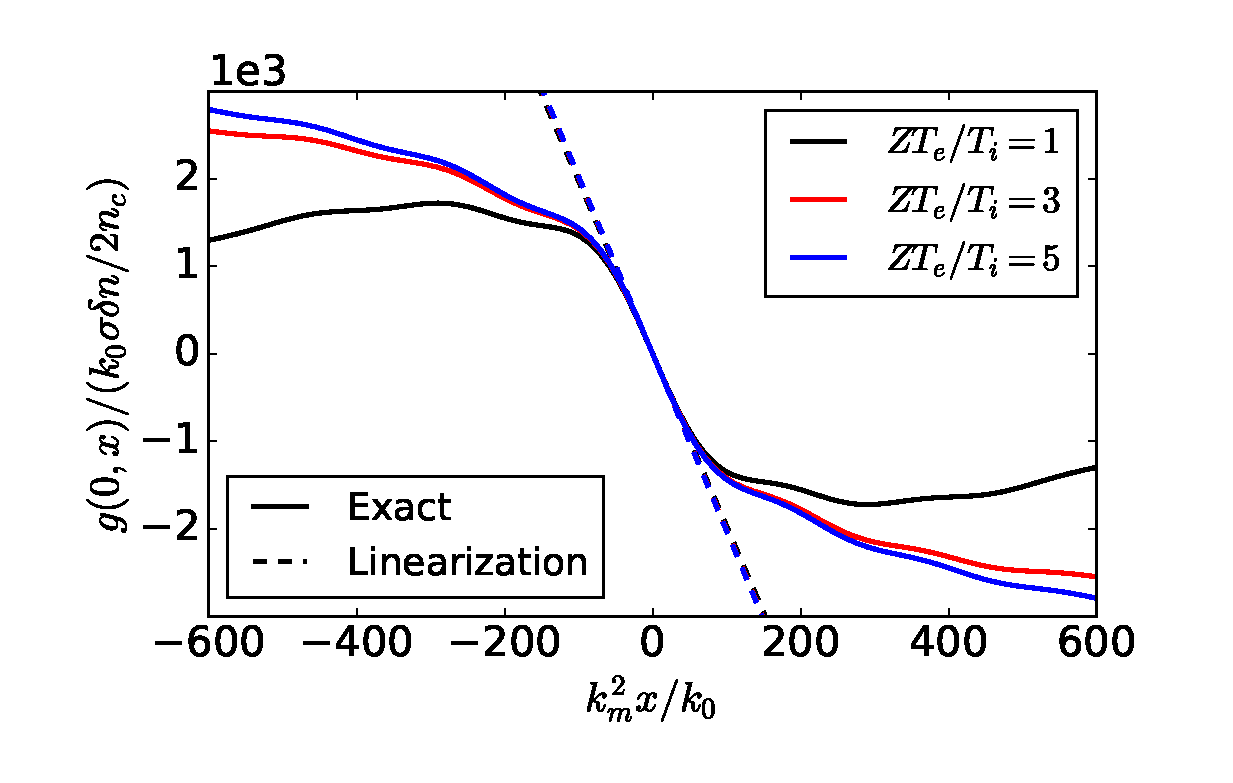
\includegraphics[width=0.49\textwidth]{int_akin_sin.eps}
 &
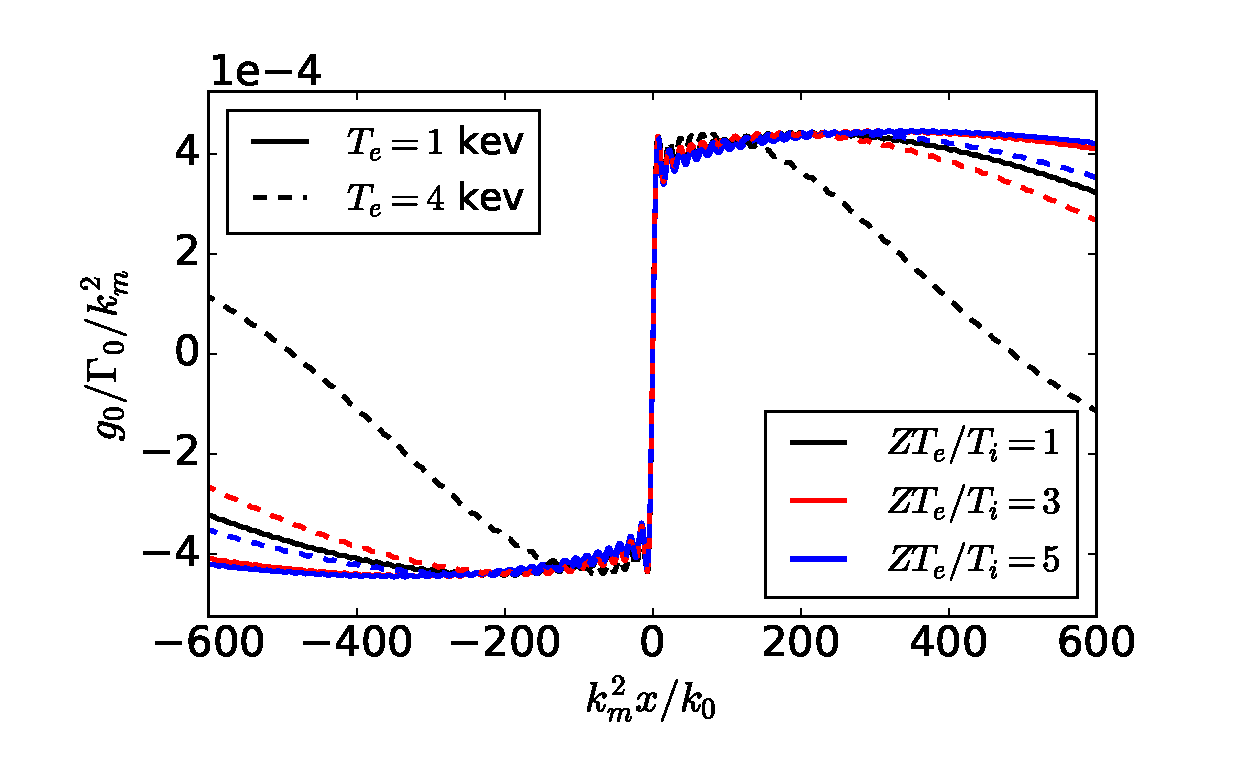
\includegraphics[width=0.49\textwidth]{int_akin_sin_D2.eps}
\end{tabular}
\caption{ \label{fig:intakinsin}
Numerical calculation of $g_0(x)$ by Eq. \eqref{eq:gain0} for $\sigma = 200 \,\mu m$ and  for various values of $ZT_e/T_i$ in the case $D=1$ (a) and $D=2$ (b). 
 }
\end{figure*}
%\begin{align}
%g(\mathbf{k}_d,x) = \frac{\partial_x I_d(\mathbf{k}_d)}{I_d(0)} %\nonumber \\
%=  \frac{-k_0}{2} \frac{ \delta n}{n_c}   \sigma^D
% \mathcal{H}^{(D)}(\mathbf{k}_d)
% \int \frac{d^Dk_s}{(2\pi)^D}    \alpha_\mathrm{r}(\mathbf{k}_s) \sin\left[{\frac{ (\mathbf{k}_d-\mathbf{k}_s)^2x}{4k_0}}  \right]\, . \label{eq:gainkd}
%\end{align}

%Making use of 
%\begin{align}
    %\int_{-2k_m}^{+2k_m}dk\sin\left[{\frac{ (k-k_s)^2x}{4k_0}}  \right]=\sqrt{\frac{2\pi k_0}{x}}\left[ \mathrm{S}\left(\sqrt{\frac{x}{2\pi k_0}} (2k_m- k_s)\right)-\mathrm{S}\left(\sqrt{\frac{x}{2\pi k_0}} (-2k_m -k_s)\right)\right]
%\end{align}
 \end{widetext}
Deriving the exact and general solution of the above equation is out of the scope of this manuscript, however, interesting results may emerge from tractable limits. 

 \subsection{Angular dependence of the  Forward Brillouin scattering}\label{sec:sp}
As the plateau width of $\alpha_r$ is much smaller than $2k_m$, \textcolor{red}{(Demonstration generale)}  we may assume, in the quadrature of Eq. \eqref{eq:g5},   $ \vert\mathbf{k}_s \vert/\vert\mathbf{k}_d\vert \le\Delta k/ \vert\mathbf{k}_d\vert \ll 1$ so that, to leading order,
\begin{align}
\partial_xI_d(\mathbf{k}_d,x)&\simeq  \frac{-k_0}{2} \frac{ \delta n}{n_c}   \sigma^D 
 \mathcal{H}^{(D)}\sin\left({\frac{ \mathbf{k}_d^2x}{4k_0}}  \right)
B(x)
\, , \label{eq:dxidtd}
\end{align}
where $B(x)$ is,
\begin{align}
B(x)&=
 \int \frac{d^Dk_s}{(2\pi)^D}    I_d(\mathbf{k}_s,x) \alpha_\mathrm{r}(\mathbf{k}_s) 
\, . \label{eq:b}
\end{align}
With $g_0(x)$ following
\begin{align}
g_0(x)&= -\Gamma_0 \int \frac{d^Dk_s}{(2\pi)^D}  \alpha_\mathrm{r}(\mathbf{k}_s) 
\sin\left(\frac{ \mathbf{k}_s^2x}{4k_0}  \right)\,  \nonumber\\
\Gamma_0&=\frac{k_0}{2}  \frac{\delta n}{n_c}
  \sigma^D \, ,
\label{eq:gain0}
\end{align}
one can easily show that $B(x)$ fulfills 
\begin{align}
d_xB = g_0(x) B(x)\, ,
\label{eq:db}
\end{align} 
and thus, for a left boundary located at $x=x_0$,
\begin{align}
B(x) = B_0\exp\left(\int_{x_0}^x g_0 \right)\, ,
\label{eq:bf}
\end{align} 
where $B_0$ is an integration constant independent of the wavevector.

Combining Eqs.  \eqref{eq:dxidtd} and \eqref{eq:bf} yields 
\begin{align}
\partial_xI_d(\mathbf{k}_d,x)&\simeq -B_0\Gamma_0
 \mathcal{H}^{(D)}\sin\left({\frac{ \mathbf{k}_d^2x}{4k_0}}  \right)
\exp\left(\int_{x_0}^x g_0 \right)
\, . \label{eq:dxidtdf}
\end{align}

Figures \ref{fig:intakinsin}(a,b) illustrate, as a function of $k_m^2 x /k_0$, the evolution of $g_0(x)$
normalized to $\Gamma_0=k_0\delta n / 2n_ck_m^2$. Note that, for $\lambda_0=2\pi/k_0=0.35\,\rm\mu m$ and $f=6.5$,  $k_m^2 x /k_0=200$ corresponds to $x\simeq 2\,\rm mm$. 
The value of $g_0$ is negative before focus (\emph{i.e.} $x=0$) and positive afterward, with  a linear behavior of the $g(0,x)$ for  $\vert k_m^2 x /k_0 \vert < 50$  independent of $ZT_e/T_i$. In both cases $D=1$ and $2$, the slope of $g_0(x)$  in the vicinity of $x=0$   decreases significantly when   $\vert k_m^2 \vert x\vert /k_0 \vert \gtrsim 50$, this occurs when the $\sin(k^2x/4k_0)$ in the quadrature of Eq. \eqref{eq:gain0} varies faster than the plateau width of $\alpha_r$, $\vert k_s/k_0\vert \lesssim 5\cdot 10^{-3}\equiv \Delta k/2$ in Figs. \ref{fig:akin}(a,b), \emph{i.e.} for $\vert x\vert \gtrsim k_0/\Delta k^2$ which gives $\vert k_m^2x/k_0 \vert  \gtrsim 60  $ in reasonable  agreement with Figs. \ref{fig:intakinsin}(a,b).
For both dimensions and $\vert k_m^2 x /k_0 \vert \gtrsim 400$, the absolute value of $g_0(x)$ vanishes faster as $ZT_e/T_i$ decreases. 

Interestingly, when $ZT_e/T_i=1$ and $T_e=4$ kev, $g_0$ become positive for $k_m^2x/k_0<-400$, \emph{i.e.} well before focus (at $x=0$). In this region,  the $\sin(k^2x/4k_0)$ in the quadrature of Eq. \eqref{eq:gain0} is minimized   where $\alpha_r$ reaches its minimum [see Fig. \ref{fig:akin}(a), $\vert k_s/k_0\vert \simeq 0.01$ for $ZT_e/T_i=1$ and $T_e=4$ kev in dashed black line]. Indeed, plugging  $\vert k_s/k_0\vert \simeq 0.01$ into $3\pi/2>k^2x/4k_0>\pi/2$ results in a positive value of $g_0$  when $1100\gtrsim \vert x\vert\gtrsim 370$, in agreement with Fig. \ref{fig:intakinsin}(a) (dashed black line).
Note that if the Forward stimulated Brillouin  scattering were to grow   and affect the pump propagation more than four millimeters before focus, a large impact on the pump propagation and its energy deposition is to be expected.

Let's momentarily consider, for illustration purposes,  the  case of a RPP beam of width $\sigma =200\,\rm\mu m$, $I_0=3\cdot 10^{14} \,\rm W.cm^{-2}$, $2\pi/k_0 = 0.35\,\rm\mu m$ and $f = 6.5$ propagating in a H$^{+}$ plasma with $n_e/n_c=0.1$,  $T_e=1$ keV and $T_i=300$ eV. In these conditions, $\delta n/n_c \simeq 7\cdot 10^{-4}$ and  for $D=1$ [see Fig. \ref{fig:intakinsin}(a)], one have $g_0(x)/\Gamma_0k_m \gtrsim 3\cdot 10^{-3}$ before focus (for $200< k_m^2 x/k_0 < 600$) so that, for  a propagation of $\Delta x = 2\,\rm mm$ (\emph{i.e.} $k_m^2 \Delta x/k_0 = 200$), the net gain is $g_0(x)\Delta x\sim 7 $. When $D=2$ [see Fig. \ref{fig:intakinsin}(b)], one obtains $g_0(x)\Delta x\sim 350 $, thus yielding substantial gain for both dimensions.

We therefore know that the Forward Brillouin may grow significantly in the plasmas  of interest here and, in order to shade light on the scattered  direction of the pump wave, we will now address the spectral behavior of Eq. \eqref{eq:dxidtdf}.

\section{Approximated and analytical formulation of the effective gain}
\subsection{The role of seed acoustic fluctuations on the growth of FSBS}
Whether $g_0$ is positive or negative,  the scattered intensity can grow following Eq. \eqref{eq:dxidtdf} ($\partial_x I_d>0$) provided that the wavevectors verify $\vert k_{x/y}\vert \le 2k_m$ and $-\sin( \mathbf{k}^2x/4k_0 ) >0$.
However, when $g_0<0$ the exponential term in Eq. \eqref{eq:dxidtdf} rapidly damp the growth, keeping $I_d$ to negligible values or, physically, close to the self sustained noise level.   
Not capture by our model, the interplay between the thermal fluctuations (assuming they represent the   appropriate seed term) and the growth of the Forward Brillouin  requires to couple the above model with a source noise  \cite[]{Yoon_2007,Ruyer_Gremillet_2013} and is out of the scope of this manuscript. 
For this study we will settle for assuming that while $g_0<0$, $I_d$ is kept to a finite seed level. 
Equation \eqref{eq:dxidtdf} will therefore be solved only in the region $g_0\ge 0$ by replacing the left boundary location  $x=x_0$ by $x=x_c$ for which $g_0(x>x_c)\ge 0$. 

Regarding the unstable modes, the most growing wavevectors verifies  $\vert \mathbf{k}\vert =k_{n\pm}$ with  $-\sin(k_{n\pm}^2x/4k_0 ) =1$,
\begin{equation}\label{eq:kn}
    k_{n\pm}^2(x) =\frac{4\pi k_0}{x} \left(2n \mp \frac{1}{2}   \right) \, .
\end{equation}
Here, $n$ is a signed  integer with  $n \cdot x /\vert x\vert\in  \llbracket 1 ,N_\mathrm{max} \rrbracket$ and  $ N_\mathrm{max}$ ensues from setting  $k_n=2k_m$ in Eq. \eqref{eq:kn},
\begin{equation}\label{eq:nmax}
    N_\mathrm{max} =\left\lfloor  \frac{k_m^2\vert x\vert }{2\pi k_0} +\frac{1}{4}   \right\rfloor \,  ,
\end{equation}
where $\lfloor u  \rfloor$ is the floor value of u. 
There is a total of $4N_\mathrm{max}$   unstable wavevectors $k_n$  which are not regularly distributed in the the initial RPP spectral width $\vert k \vert< 2k_m$ since $k_n\sim n^{1/2}$. 

\subsection{Forward Brillouin-unstable region after the focal plane}
\begin{figure}[!]
\begin{tabular}{cc}
\includegraphics[width=0.49\textwidth]{sin2.png}\\
\end{tabular}
\caption{ \label{fig:sin2} Illustration of $-\sin\left({\frac{ k^2x}{4k_0}}  \right)$ as a colormap.}
\end{figure}
We may now address the region $x>0$ for which Figs. \ref{fig:intakinsin}(a,b) evidence $g_0>0$.
As $x$ grows starting from  $x=0$,  $\partial_x I_d$ starts to be positive  first for  $\vert k_{y/z} \vert= 2k_m$  if the $-\sin$ of Eq. \eqref{eq:dxidtdf}, illustrated in Fig. \ref{fig:sin2}, is positive, \emph{i.e.} $2\pi>4k_m^2x/4k_0>\pi$ and  when 
\begin{equation}\label{eq:xc}
x_1^- = \frac{\pi k_0 }{k_m^2}  <x < x_1^+ = \frac{2\pi k_0 }{k_m^2} \, .
\end{equation}
We will therefore,  use $x_0\equiv x_c=x_1^-$ during the resolution of Eq. \eqref{eq:dxidtdf}. 

Moreover, as illustrated in Fig. \ref{fig:sin2}, the first most unstable mode, $k_1(x)$, enters in the  RPP spectral width, $\vert k \vert< 2k_m$, when $k_1(x)=2k_m$ so that 
$x=3\pi k_0 /2k_m^2=(x_1^++x_1^-)/2$. As $x$ increases and become larger than $x_1^+$, more and more mode verifies $\vert k_{y/z} \vert= 2k_m$, and the number of unstable wavevectors increases linearly, following Eq. \eqref{eq:nmax}.

A simple analytical formulation of the scattered  intensity amplification is reachable  when assuming $g_0$ constant. Such assumption is fairly well verified in the case $D=2$ as $g_0$ presents a plateau [see Fig. \ref{fig:intakinsin}(b)]  around $g_0/\Gamma_0k_m^2 \sim 4\cdot 10^{-4}$  in the region $k_m^2x/k_0  \lesssim  600 $ ( $  \lesssim  180 $) when $T_e=1$ keV ($T_e=4$ keV). 
As for $D=1$, the replacement of  $g_0$ by a constant ($g_0/\Gamma_0k_m\sim 3\cdot 10^{-3}$), although as shown subsequently enlightening, is more questionable when  $T_e=1$ keV and wrong for $T_e=4$ keV.

\begin{figure*}[!]
\begin{tabular}{cc}
(a) $D=1$, $k_m^2x/k_0=212$
& (b) $D=2$, $k_m^2x/k_0=212$\\
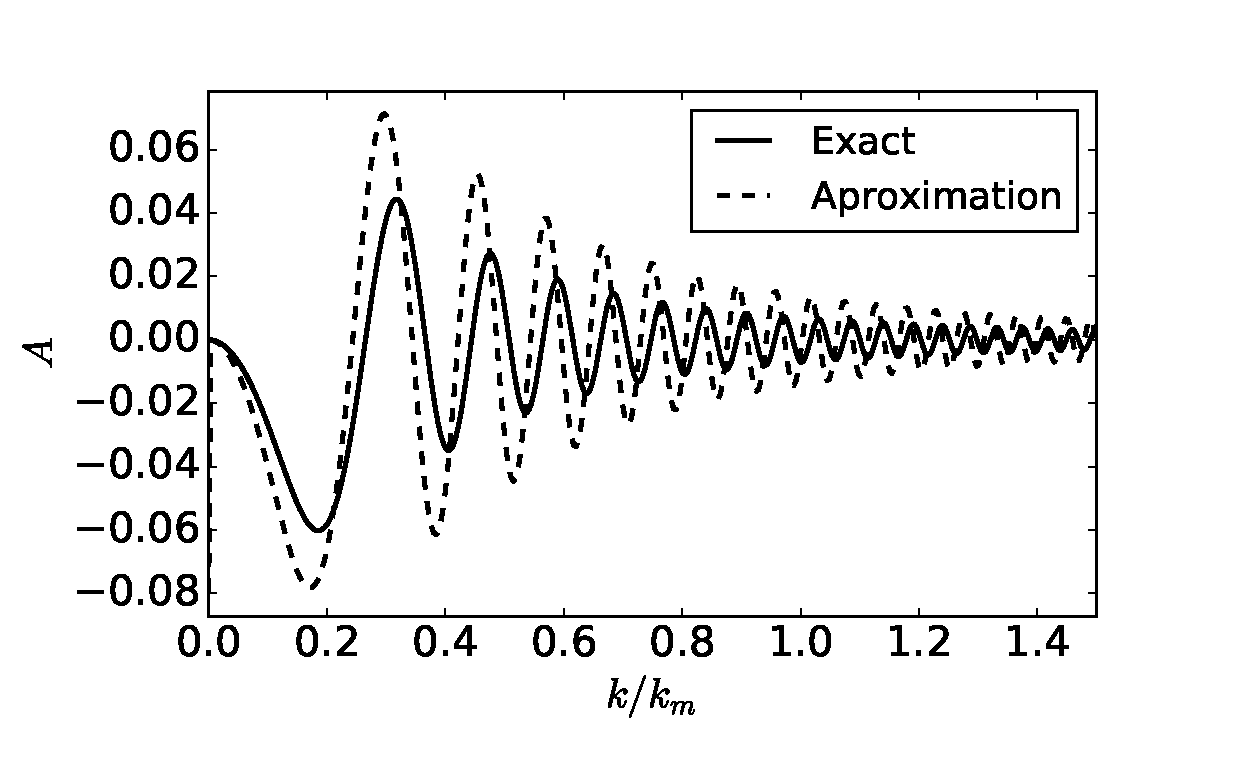
\includegraphics[width=0.35\textwidth]{AD1.eps}
&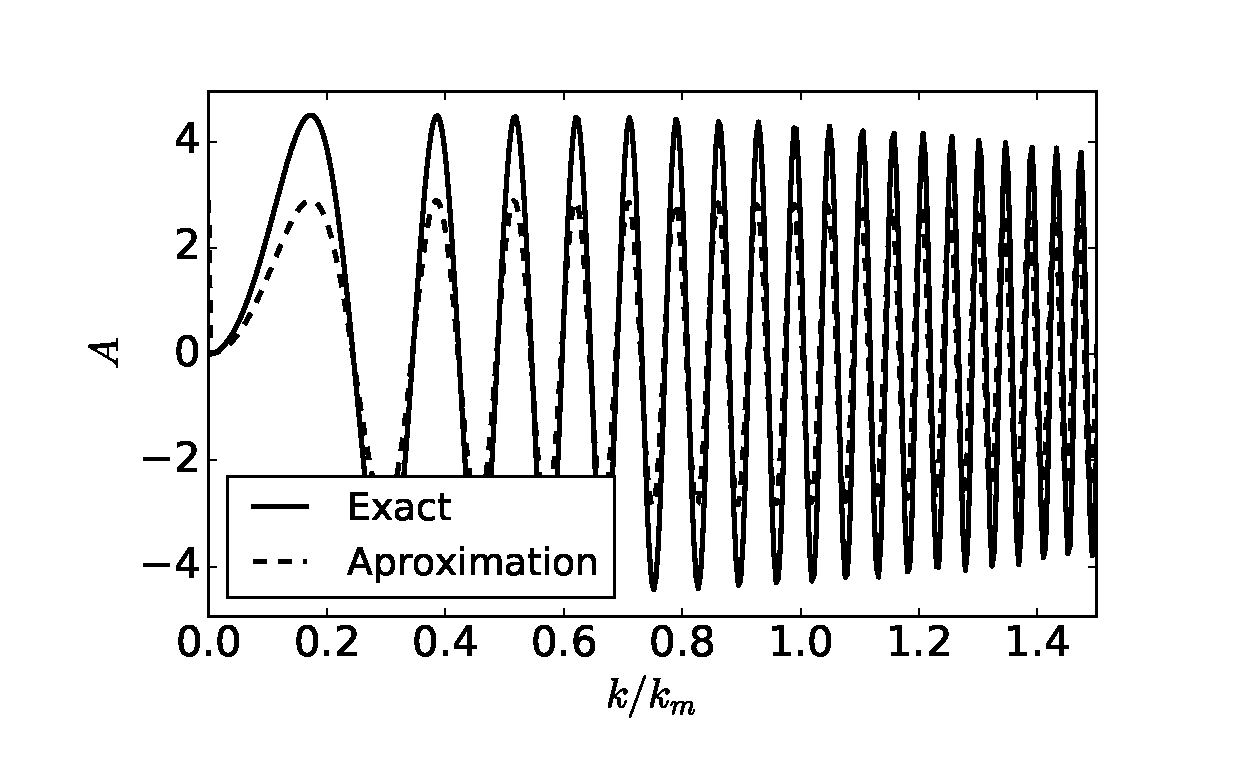
\includegraphics[width=0.35\textwidth]{AD2.eps}\\
(c) $D=1$ 
& (d) $D=2$\\
\includegraphics[width=0.35\textwidth]{AxkD1.png}
&\includegraphics[width=0.35\textwidth]{AxkD2.png}
\end{tabular}
\caption{ \label{fig:ical}
Evolution of $\mathcal{I}$ as defined in Eq. \eqref{eq:icaldef} for $D=1$ (a,c) and $D=2$ (b,d) from the exact resolution of Eq. \eqref{eq:dxidtd} at $x = 2$ mm as plain lines  (a,b). 
The approximation of Eq. \eqref{eq:ical} with $\Tilde{g_0}/\Gamma_0k_m^{D} = 3\cdot 10^{-3}$  and $2\cdot 10^{-4}$ for $D=1$ and $2$ respectively in (c,d) are also superimposed on (a,b) as dashed lines and as circles located at $k=k_n$ defined by Eq. \eqref{eq:kn}. 
The parameters used are $I_0 = 3\cdot 10^{14}\, \rm W.cm^{2}$, $2\pi/k_0=0.35 \,\rm\mu m$, $f=6.5$, $T_e =1\,\rm  keV$, $ZT_e/T_i=3$ and $\sigma=200\,\rm\mu m$  (\emph{i.e.} $\Gamma_0=1.2\sigma^{D-1}$).
}
\end{figure*}
Hence for $g_0\equiv \Tilde{g_0}$ constant and $x>x_c$, Eq. \eqref{eq:dxidtdf} becomes
\begin{align}
   \partial_x I_d&=-B_0\Gamma_0 \mathcal{H}^{(D)}(\mathbf{k}_d)e^{  \Tilde{g_0}(x-x_c)} 
    \sin\ \left(\frac{\mathbf{k}_d^2x }{2k_0}  \right)   \, , \label{eq:idtd1} 
    %\\ A_0 &= \int \frac{d^Dk_s}{(2\pi)^D}    \alpha_\mathrm{r}(\mathbf{k}_s) \, .\label{eq:a0}
\end{align}
For simplicity, we also assumed $I_d(x=x_c)=I_{d,0}$ independent of $\mathbf{k}$, so that following, Eq. \eqref{eq:bf}, $B_0 = I_{d,0}A_0$.
After resolution, defining $\mathcal{I}$ though
\begin{align}
    \frac{I_d(\mathbf{k}_d,x)}{I_{d,0}}-1& \simeq
   \mathcal{I}(\mathbf{k}_d,x)
   \exp\left(\int_{x_c}^{x}g_0\right)
    \, , \label{eq:icaldef} 
\end{align}
we obtain
\begin{align}
    \frac{I_d(\mathbf{k}_d,x)}{I_{d,0}}-1& \simeq
   \mathcal{I}(\mathbf{k}_d,x)
   e^{\Tilde{g_0}(x-x_c)}
    \, , \label{eq:idf} \\
    A_r &= \int \frac{d^Dk_s}{(2\pi)^D}    \alpha_\mathrm{r}(\mathbf{k}_s) \, ,\label{eq:ar}\\
    \phi(\mathbf{k}) &= \arctan \left(  \frac{\mathbf{k}^2}{4k_0\Tilde{g_0}}\right)\, , \label{eq:phi}
\end{align}
with 
\begin{widetext}
\begin{align}
    \mathcal{I}(\mathbf{k}_d,x)& \simeq
   \frac{
   -A_r  \mathcal{H}^{(D)}(\mathbf{k}_d)
   }{
 % \left[
   \sqrt{\frac{\Tilde{g_0}^2}{\Gamma_0^2}  +\frac{\mathbf{k}_d^4 }{16k_0^2 \Gamma_0^2}}
    %\right]^{-1}
    } 
    \left[
    \cos\left( \frac{\mathbf{k}_d^2x }{2k_0}  -\phi(\mathbf{k}_d) \right) 
   -e^{-\Tilde{g_0}(x-x_c)}\cos\left( \frac{\mathbf{k}_d^2x_c }{2k_0}  -\phi(\mathbf{k}_d) \right) 
    \right]
    \, . \label{eq:ical} 
\end{align}
\end{widetext}
Figures \ref{fig:ical}(a,b) compares the spectral form factor of the final scattered intensity, $\mathcal{I}$ as defined by Eq. \eqref{eq:icaldef}, computed by numerical integration of Eq. \eqref{eq:dxidtdf} (plain lines) and through the approximation of Eq. \eqref{eq:ical} (dashed lines). A good quantitative agreement is evidenced for  both dimensions in the peak position and in their amplitude when $D=2$. 
Regarding $D=1$, the approximation $\int g_0\simeq  \Tilde{g_0} x$ is, as stated above,   less appropriate resulting in an overestimate of Eq. \eqref{eq:ical} of roughly $\sim 50\%$. 
The peak positions, as predicted by Eq. \eqref{eq:kn} in circles, agrees very with the reference curve showing that the first  $\cos$ of Eq. \eqref{eq:ical} is very close to the $\sin(k^2x/k_0)$ of Eq. \eqref{eq:dxidtdf}.
The derivation of Eq. \eqref{eq:dxidtdf} required the assumption $\vert \mathbf{k}\vert\gg \Delta k $, with  
$\Delta k/k_m \simeq 6.5\cdot 10^{-2}$ for $f=6.5$ (see Fig. \ref{fig:akin}(a) showing $\Delta k/k_0 \simeq 5\cdot 10^{-3}$ for $T_e=1$ keV), thereby, the validity of the region  $\vert k\vert /k_m \lesssim 0.5$ in Figs. \ref{fig:ical}(a-c) is doubtful. 

According to the the spatial evolution of $\Tilde{I}$ illustrated in Figs. \ref{fig:ical}(c,d), only large wavevectors ($k_m\lesssim \vert k\vert<2k_m$) are amplified close to the focal plane, $k_m^2x/k_0\lesssim 20$. Afterward, as the number of unstable modes grows linearly with $x$ [see Eq. \eqref{eq:nmax}],   the region  $\vert k\vert<k_m$ becomes unstable. As all perturbative models, our predictions holds as long as the scattered intensity remains negligible compared to the pump wave, otherwise, non linear saturating effects such as pump depletion are to be expected leading to the stop of the $I_d$-growth. Provided such saturation occurs around $k_m^2 x/k_0\sim 20-50$, only large wavevectors will have been amplified before saturation leading to the redistribution of the pump energy on the edges of the initial propagating cone ($\theta\le  2k_m/k_0$), thus deforming significantly  the intensity pattern. Such phenomenon would result in more energy deposition on the sides of the beam. 

On the contrary, if the Forward Brillouin saturates at $k_m^2x/k_0\gtrsim 100$ for the plasma parameters of  Figs. \ref{fig:ical}(a-c), two different behaviors are predicted depending on the dimension. When $D=1$, Figs. \ref{fig:ical}(a,c) indicate that mainly low wavevector modes ($\vert k\vert<k_m$) are amplified, leading to the narrowing of the propagating cone angle and more energy deposition on the laser main axis.
Indeed the square root in the denominator of Eq. \eqref{eq:ical} damps $\mathcal{I}$ for wavevectors larger than $k\gtrsim \kappa = 2(k_0\Tilde{g_0})^{1/2}$, which for  $D=1$ yields $\kappa/k_m \simeq 0.4 $, thus resulting in the decrease of $\mathcal{I}$ at large wavevectors. Regarding  $D=2$, we obtain $\kappa/k_m \simeq 1.9 $ which explains that the $\mathcal{I}$-peaks  values remain fairly independent of $\mathbf{k}$ [see Figs. \ref{fig:ical}(b,d)]. In this case, the majority of the modes presents comparable amplification factor however,  most of them are located in $\vert k_n\vert >k_m$, probably leading to the scattering of the pump intensity on the edges of the cone propagating angle.

We will now extract an effective spatial growth rate from the above equation. Defined as $\Gamma = \partial_x \log(I_d)$,  it may be recast   as 
\begin{equation}
  \Gamma \simeq \frac{
  \partial_x [\mathcal{I}e^{\Tilde{g_0}(x-x_c)} ]
  }{
  \mathcal{I}e^{\Tilde{g_0}(x-x_c)} 
  }
  \, ,\label{eq:gdef}
\end{equation}
provided $I_d/I_{d,0}\gg1$.
The use of Eqs. \eqref{eq:dxidtdf} and \eqref{eq:ical}  gives,
\begin{equation}
  \Gamma(\mathbf{k},x) \simeq  \mathcal{H}^{(D)}(\mathbf{k}) \left[ 
  \frac{\mathbf{k}^2}{ 4k_0 } \tan\left(\frac{\mathbf{k}^2x}{4k_0}-\phi\right)
  +\Tilde{g_0}
  \right]
  \, .\label{eq:g1}
\end{equation}
Restricting the analysis to the peaks of $\partial_x I_d(\mathbf{k})$  at $\mathbf{k}=\mathbf{k}_{n\pm}$ [see Eq. \eqref{eq:kn}], and since $\vert \tan(\mathbf{k}_{n\pm}^2x/4k_0)\vert\rightarrow \infty$, we finally obtain the surprisingly compact formula,
\begin{equation}
  \Gamma[\mathbf{k}_n(x)] \simeq  2\Tilde{g_0}
  \, .\label{eq:gf}
\end{equation}
The simplest way to estimate the growth of FSBS seems  therefore to consist in scattering randomly the pump wave into a  seed beam in one of the directions predicted by Eq. \eqref{eq:kn}  depending  on the position after focus  and 
following an exponential growth rate of parameter $2\Tilde{g_0}$ [as estimated either though dedicated numerical calculations or by arbitrarily setting $\Tilde{g_0}$ to $g_0(k_m^2 x/k_0 =200 )$ for example].

\section{Conclusions and perspectives}
We presented a model which  aims to capture, or at least to estimate, the amount of scattered energy of an RPP laser pulse off acoustic and  large wavelength density fluctuations. The kinetic response of the plasma  to the driven perturbations  seems essential for understanding the growth of the diffused wave. 
The resulting formula could pinpoint the rear focal plane region as FSBS-unstable but also indicates that a growth may occur far before focus  provided the electrons are hot enough.  
For highly unstable systems, depending on the pump depletion location and on the dimension, two different behaviors may arise such as the scattering of the pump energy on the edges or in the center of the initial propagating cone, thus modifying  the expected intensity pattern after focus and the subsequent energy deposition.

Among the assumptions that retrain the range of this study, one may think of the asymptotic kinetic plasma response (Sec. \ref{sec:drake}) narrowing our predictions to long time behavior or pump waves without spectral dispersion. 
We could also mention the large wavelength Taylor developments use in Sec. 
\ref{sec:sp} which  leaves a vagueness regarding the long wavelength behavior. Finally, the interplay of FSBS with other parametric instabilities such as stimulated Raman scattering or CBET is also of clear interest. 


\section*{Acknowledgements}
We acknowledge important discussion with M. Grech.  We also admit the role of the confinement following the COVID19 plague for forcing us to take the time to finalize this theoretical work. This work has been done under the auspices of CEA-DAM. 
% and the simulations were performed using HPC resources at TGCC/CCRT and CEA-DAM/TERA.
\bibliography{biblio}
\end{document}
